\documentclass[fleqn]{article}
\usepackage{xcolor, etoolbox}
\usepackage{amsmath}
\usepackage{graphicx}
\usepackage{wrapfig}
\usepackage[margin=0.5in]{geometry}
\usepackage{caption}
\usepackage[font={color=black!30!white},figurename=Fig.,labelfont={it}]{caption}
\usepackage{tabto}
\usepackage{hyperref}

\title{OpenCV Computer Vision 1 Notes}
\date{3-25-2020}
\author{Maxwell Li}

\begin{document}
  % This is what sets the page number color
  \makeatletter % change only the display of \thepage, but not \thepage itself:
  \patchcmd{\ps@plain}{\thepage}{\textcolor{black!20!white}{\thepage}}{}{}

  % This sets the theme for the page
  \color{black!20!white}
  \pagecolor{black!80!white}

  \maketitle
  \tableofcontents
  \setcounter{secnumdepth}{0}
  \pagenumbering{arabic}
  \newpage

  \section{\textbf{Week 1: Getting Started with Images}}
    \subsection{Introduction}
    Some things we will learn\\
    \quad - What is color?\\
    \quad - How does a camera see an image?\\
    \quad - How to read/write images?\\
    \quad - How to manipulate pixels?\\
    \quad - Alot more!

    \subsection{How is An Image Formed}
    Throughout history the phenomena of imaging has been explored by many ancient civilizations. The most used primitive form of a camera that has been used was the pinhole camera. The pinhole camera works by taking the light waves that bounce off of an object and projecting them through a small hole.

    \begin{figure}[h]
      \centering
      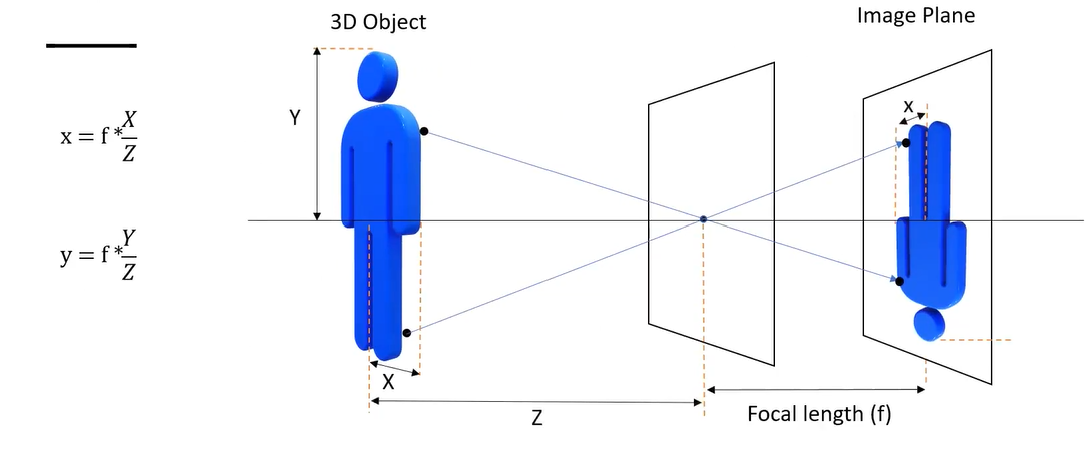
\includegraphics[width = 250pt]{pinholecamera.png}
      \caption{PinHole Camera Example}
      \label{fig: Pinhole Camera}
    \end{figure}

    %

    \subsection{Image Formation}
    Inside of a camera there is a sensor that is a large grid of nodes. These nodes are what eventually become ``pixels'''. Each node on the sensor gets a value between 0 and 255 which represents the digital grayscale image. The value for each node is determined by the strength of the light that hits it. The stronger the light the closer the value is to 255 as 255 is white and 0 is black. Each pixel is essentially an 8 bit representation of the intensity of the light at that position on the sensor.

    \begin{figure}[h!]
      \centering
      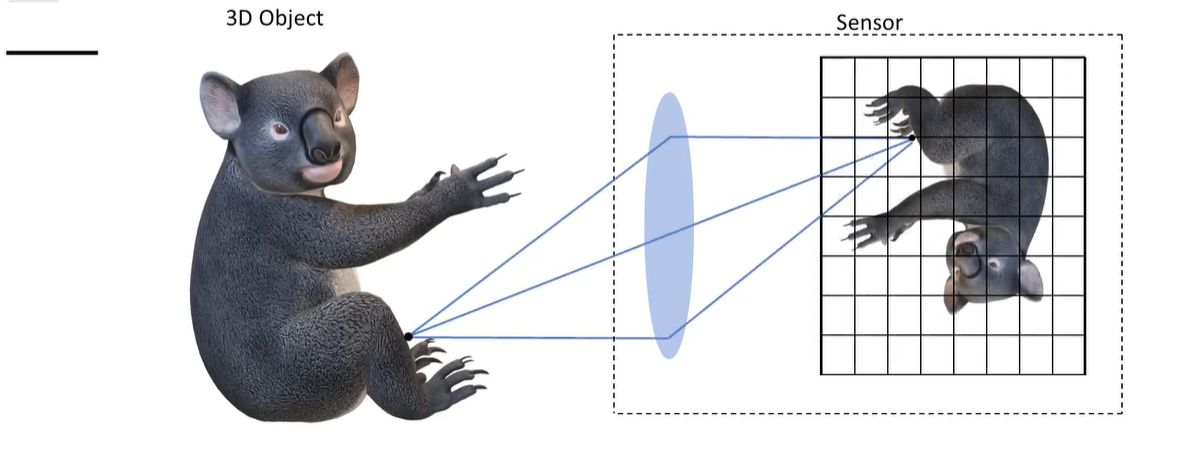
\includegraphics[width=250pt]{koala.png}
      \caption{Greyscale Digitalization }
      \label{fig: Greyscale Representation of an Image}
    \end{figure}



    \newpage
    \clearpage
    \subsection{Bayer Pattern}
    Every pixed only records one color: red, green, or blue. The human eye is much more sensitive to green light than blue or red. The full RGB Image is then formed through a process called demosaicing where 2 two missing values from each pixel are calculated from the neighbouring pixels\\
    \textbf{For example:} If a pixel records the red value, based on the pixels around it the pixel will interpolate what the correct hue for the 2 missing colors.

    \begin{figure}[h!]
      \centering
      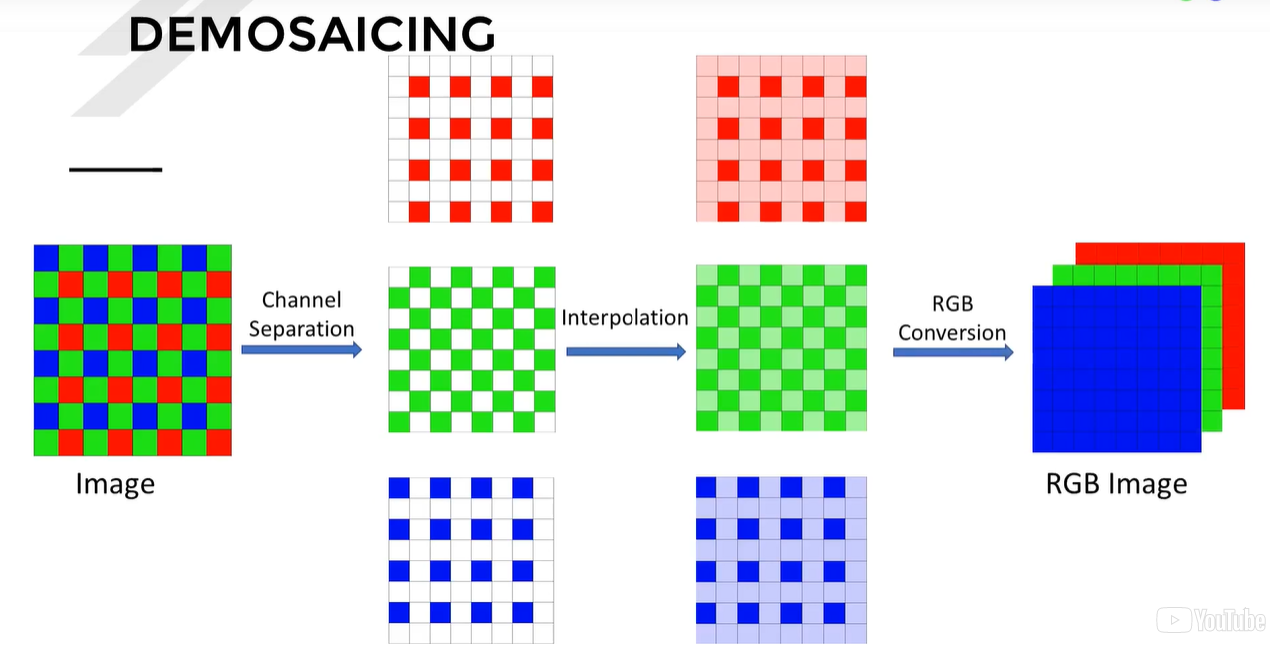
\includegraphics[width=550pt]{demosaicing.png}
      \caption{Process of Demosaicing}
      \label{fig: How the total RGB Image is found through demosaicing}
    \end{figure}

    \subsection{Image Format}
    Once a RGB image is created, they are typically stored and compressed as either Joint Photographic Expert Group (JEPGs) or Portable Network Graphics (PNGs).

    \subsubsection{Image Storage}
    Within a JPEG file the image is broken up into two parts. There is the Image Header and the Data.\\
    \tab - Image Header\\
    \tab\tab - Width\\
    \tab\tab - Height\\
    \tab\tab - No. of channel\\
    \tab\tab - Color Profile\\
    \tab\tab - No. of bits per pixel\\
    The second part is the data which actually contains the RGB values

    \subsection{Image in OpenCV}
    When an image is first read in openCV the image is decompressed and stored in a standardized format. All images are stored into the \textbf{Mat Class} if the C++ version is being used, or a \textbf{Numpy array} if Python is being used.

    \subsubsection{Mat Class}
    The Mat class is similar to a JPEG in structure but the difference is that instead of using RGB values it used BGR. It uses bgr because of historic reasons, aka that is how they initially did it and it makes no sense to back through and change all of the backend code now.

    \newpage
    \clearpage
    \section{Week 1: Reading/Writing/Modifying Images in OpenCV}
    \subsection{Image Formats}
    OpenCV can use two different formats, JPEG and PNG

    \begin{wrapfigure}{r}{400pt}
    \centering
    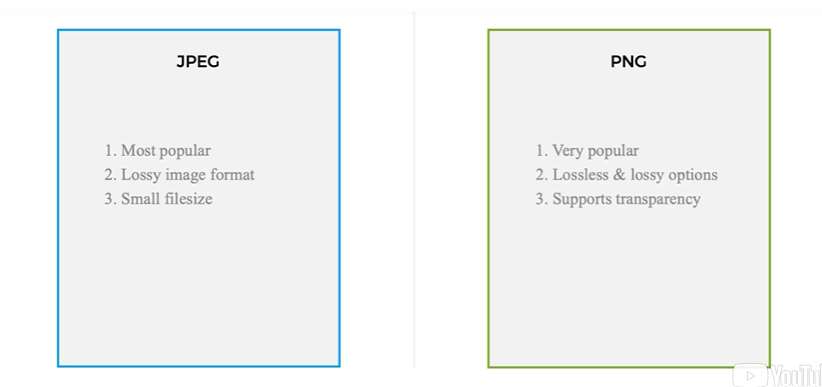
\includegraphics[width=325pt]{jpegvspng.png}
    \caption{\label{fig:jpegvspng}JPEG vs PNG.}
    \end{wrapfigure}


    \subsubsection{JPEG}
    1) Most Popular\\
    2) Loss in image format\\
    3) Small Filesize
    \subsubsection{PNG}
    1) Very Popular\\
    2) Lossless and lossy options\\
    3) Supports transparency\\ \\ \\
    \subsubsection{Transparent Images}

    \begin{wrapfigure}{r}{300pt}
    \centering
    \includegraphics[width=200pt]{Transparentimage.png}
    \caption{\label{fig:Transparentimage}RBG vs Transparent RGB.}
    \end{wrapfigure}
    Contains all three regular channels (Red, Green, Blue) and also contains an `Alpha' channel that acts as a mask (255 or 0). The value that is put into the alpha channel is determined by the Opacity of the pixel. If the pixel is ``Transparent'', then there will be a 0 for that pixel in the Alpha channel. If the pixel is not ``Transparent'', then it will recieve a value of 255.\\
    ***Note: Alpha channels do not neccesarily have to be binary. They can be tertiary or higher if for some reason that kind of masking is wanted/needed. Aka, there can be partial transparencies

    \subsection{Reading The Image (Week One: Getting Started With Images)}
    To load an image through OpenCV use the \textbf{imRread} function. This function is able to handle most, if not all of the image types that you may want to upload (these include JPEG, PNG, etc)

    \subsubsection{Function Syntax: cv2.imread}
    \textbf{$loaded image = cv2.imread(filename, flags)$}\\
    \tab this function (imread) will return the image as a matrix or None if something happened that it was not able to resolve.
    \tab This function has \textbf{two arguments}:\\
    \tab \tab 1) The \textbf{path} of the image file: this can be absolute or relative and is a mandatory argument\\
    \tab \tab 2) \textbf{Flags:} -1, 0, or 1. ***DEFAULT IS ONE***\\
    \indent \indent $cv2.IMREAD\_UNCHANGED$ or -1: Loads an image including the alpha channel (unchanged)\\
    \indent \indent   $cv2.IMREAD\_GRAYSCALE$ or 0: Loads the image in grayscale\\
    \indent \indent  $cv2.IMREAD\_COLOR$ or 1: Loads a color image and throws out transparency\\

    \newpage
    \clearpage
    \subsection{Manipulating Pixels (Week One: Getting Started With Images)}
    \subsubsection{Accessing Values}
    \indent Since the openCV returns things as a matrix of values, you can just access them using the subscript notation of matricies.\\
    IMPORTANT: Numpy saves the matrix in row column format which is the opposite of x,y format. For example if you want to access the pixel to the right of the top left instead of (1,0), which is the cartesian representation of it, it would be [0,1]. This is an important distinction as it will allow you to actually access the correct variables.\\

    \begin{center}
      $print(testImage[0,0])$
    \end{center}


    \subsubsection{Modifying Values}
    Just use a normal python $=$ operation for this. You can either modify a single value or a whole region...that is next\\
    There are a few reasons why people would want to change the values of the pixels. For one, if there is a known issue with the image or a known change that the user might want to change, they need to be able to access and modify the values. For example maybe the edges of the image are blurry so you just set them all to 0 so that there are no false positives.

    \begin{center}
      $testImage[0,0]=200$\\
      $print(testImage)$
    \end{center}

    \subsection{Manipulating Groups of Pixels (Week One: Getting Started With Images)}
    \subsubsection{How To Access A Region}

    \begin{center}
      ROI - Region of Interest\\
      $test\_roi = testImage[0:2,0:4]$\\
    \end{center}

    This code will return a resulting matrix the is 2 rows tall, and 4 columns long. This is a bit counterintuitive because if you count up from 0 (where subscript position starts), and go to the last number then both dimensions are missing 1 element. This is because python is inclusive of the lower bound but non inclusive of the upper bound. \\
    0:2 tells python, hey! Look in this matrix and take out rows 0 and 1, stop before two, and also take columsn 0, 1, 2, 3 and stop before four. Now stich this all together into a matrix and return it! This way the programmer can select a specific part of the iamge that they are interested in using aka, Region of Interest.\\
    To set a region of interest to a specific value all you have to do is take the region, and use the equals operator.

    \begin{center}
      $testImage[0:2,0:4] = 111$
    \end{center}

    \subsection{Displaying An Image}
    Previously learned were the ways that you could display the matrices that made up a specific image and see the values that they contained. Also learned were the ways to modify a pixel or a ROI (Region of Interest). All of this however is pretty much useless as it isn't really possible to visualize a whole picture by just looking at the matricies. There is the need to actually display the image and when using python that is done with Matplotlib.\\
    Matplotlib is a python library for data visualization and does a pretty good job as it. As the name implies, it is a library for plotting math related things. Matplotlib can be installed with a simple, \textbf{pip install matplot lib}. Make sure that you are on the virtualenv that you want to use it for (personally i just install everything system wide I know it is not the right way to do it but it is the way that I do it for ease of use).

    \subsubsection{Function Syntax: plt.imshow() vs cv2.imshow()}
    \indent \textbf{Matplotlib}\\
    \indent \indent - The matplot lib version of the function only has 1 mandatory argument, which is the image in the form of a matrix. A good practice is to also incluse the colorbar() function with it as well as it show a gradient colorbar based on the values.

    \begin{center}
      plt.imshow(matrix)\\
      matrix - Image to be displayed
    \end{center}

    \newpage
    \clearpage

    \textbf{OpenCV}\\
    \indent \indent - The OpenCV version of the function is similar to the Matplotlib version but where it differs is that it opens a separate window to view the image in. This version requires you to have OpenCV installed locally on your computer to run as it uses OpenCV packages.



    \begin{center}
      cv2.imshow(window name, matrix)\\
      \textbf{Read the image:} $boy = cv2.imread(data\_path + ``/images/boy.jpg'')$\\
      \textbf{Display the image using imshow: } $cv2.imshow("Boy", boy)$\\
      \textbf{Wait for user to press a key: } $cv2.waitKey(0)$\\
      \textbf{Destroy the window: } $cv2.destroyAllWindows()$\\
      ***These extra methods will be gone over in the next section***
    \end{center}

    \subsection{Addition Display Utility Functions (OpenCV)}
    \subsubsection{cv2.namedWindow}
    This function creates a display window with a specific name. The name provided is the first argument of the function. The second is a flag that determines whether or not the window can be resized. \\
    The two flags are \textbf{cv2.WINDOW\_NORMAL}, which will all the window to be resized to fit the image that is sent to it, or \textbf{cv2.WINDOW\_AUTSIDZE} which is the default if nothing is sent.
    \subsubsection{cv2.waitKey}
    This function can be used in image and video processing. The only argument that it takes is the milliseconds to wait for a key press. For example if you sent it 100 then it will wait for a key to be pressed for 100ms and proceed if the time has passed or the key has been pressed. If a 0 is passed in then it will wait indefinently until a key is pressed
    \subsubsection{cv2.destroyWindow}
    This function is pretty self explanatory. The only parameter that it takes is the window name. It will then destroy the window
    \subsubsection{cv2.destroyAllWindows}
    Just like destroywindow() except it destroys all windows.

    \subsection{Saving an Image}
    To save an image to the disk use a function called imwrite from the cv2 library.
    \subsubsection{Syntax}
    \begin{center}
      $cv2.imwrite("test.jpg", testImage)$\\
      \textbf{Parameter 1:} is the filename to be saved as, if you would like to save it as a PNG then add a .png if you want it to be saved as a JPEG then save it as a .jpg\\
      \textbf{Parameter 2:} is the matrix that you want to store to the new image file that is going to be created. \\
      There are more params that can specify the compression quality and others but they don't really matter. If you want to find out more about it just look at the documentation online.
    \end{center}

    \newpage

    \subsection{Color Images}
    This will go over how to read a color image and it's properties. \\
    To read a colored image you will still use the \textbf{cv2.imread()} function. The only difference between reading colored and non color images is that now if you check the ``shape'' of the matrix you will see that it has a 3rd dimension that is either 3 or 4. 3 for normal RGB (remember each channel is a color) or it will have 4, the 4th being the channel for transparency.

    \subsubsection{Image Channels}
    If you read in a colored image using \textbf{cv2.imread()} and then print it using the \textbf{plt.imshow()} you will see that the image is inverted. This is because OpenCV as previously discussed handles RGB as BGR. If you use the \textbf{OpenCV imread} function then it knows in what order to interprett those channels. Unfortunately Matplotlib doesn't understand the order which is why I think that it just makes more sense to use the OpenCV show function. It allows more flexability with the movable and possibly resizable window and also integrates seamlessly with OpenCV, as it should. You would think that they would all just standardize the data on one format but no, everyone wants to do it their own way and doesn't want to standardize...sigh. One day these companies will learn.\\
    \textbf{Note:} If for some reason you still feel compelled to use the Matplotlib (if you are I truly don't understand why please shoot me a message on github), then you can simply reverse the order of the last dimension of the matrix. That will convert the RBG to BGR...just use OpenCV...there is no point to go through the hassle...please.

    \subsubsection{Accessing Individual Channels}
    When wanting to pring the individual channels out and seeing what the image looks like just use the imshow method (please us cv2). The way to do this is remember that at the end of the day it is a python numpy array and that there are 3-4 channels on that last dimension of the array.
    \begin{center}
      \textbf{Code Examples of How to Show 3 channel subplots}\\
      plt.subplot(131);plt.imshow(img[:,:,0]);plt.title("Blue Channel");\\
      plt.subplot(132);plt.imshow(img[:,:,1]);plt.title("Green Channel");\\
      plt.subplot(133);plt.imshow(img[:,:,2]);plt.title("Red Channel");\\
    \end{center}
    Keep in mind that this is not doing \textbf{anything fancy}... this is
    just basic accessing of arrays. Don't get too caught up with it. You are just selecting which part of the 3rd dimension to use (one is R, one is G, one is B). To really quickly explain the subplot function:
    1 row, 3 columns, position (1) $\rightarrow$ 131\\ \\

    Another way to split the image up into the separate components would be to use the cv2.split function.

    \begin{center}
      $\#$ Split the image into the B,G,R components\\
      b,g,r = cv2.split(img)\\[0.25in]

      $\#$ Show the channels\\
      plt.figure(figsize=[20,5])\\
      plt.subplot(141);plt.imshow(b);plt.title("Blue Channel");\\
      plt.subplot(142);plt.imshow(g);plt.title("Green Channel");\\
      plt.subplot(143);plt.imshow(r);plt.title("Red Channel");\\[0.25in]

      $\#$ Merge the individual channels into a BGR image\\
      imgMerged = cv2.merge((b,g,r))\\
      $\#$ Show the merged output\\
      cv2.imshow("Merged Output", imgMerged[:,:,:])\\[0.25in]
    \end{center}
    \textbf{Note:} I did make a change to the lesson code here. The lesson code uses the plt.imshow method which takes RGB, not the BGR values that have been merged. Instead of wasting time and in the future making a mistake by not flipping the channels, I changed it to the cv2 imshow which you should use as it integrates better.

    \newpage

    \subsection{Images the Alpha (fourth) Channel}
    The best way that I can relate the alpha channel metaphorically would be like a 6th sense.  The three other channels are like the 5 senses of color and the Alpha Channel is the Fourth Channel (see the comparison to the sixth sense here). This is an original metaphor that I came up with so I am pretty stoked about it. Here is the code to use the alpha channel through OpenCV.

    \subsubsection{Example: }
      \begin{center}
        \# Path of the image to be read\\
        $image\_path = data\_path + ``images/panther.png''$ \\[0.25in]

        \# read the iamge\\
        \# the example passes a flag of -1 so that the image is read as is but to code correctly we should use the created flag for readability. \\
        $img\_png = cv2.imread(image\_path, cv2.IMREADUNCHANGED)$ \\[0.25in]

        \# First 3 channels will be combined to form BGR image
        \# Mask is the alpha channel of the original image
        imgBGR = imgPNG[:,:,0:3]
        imgMask = imgPNG[:,:,3]
        plt.figure(figsize=[15,15])
        plt.subplot(121);plt.imshow(imgBGR[:,:,::-1]);plt.title('Color channels');
        plt.subplot(122);plt.imshow(imgMask,cmap='gray');plt.title('Alpha channel');
      \end{center}

      \begin{figure}[h]
      \centering
      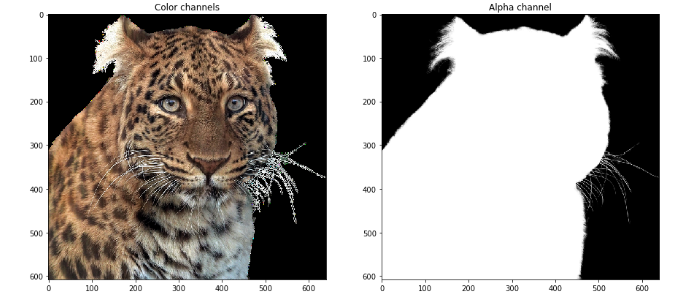
\includegraphics[width=500pt]{alphamask.png}
      \caption{\label{fig:alphamask}Example of a binary alpha mask.}
      \end{figure}

      I have learned one possible advantage to using Matplotlib which is why I kept this example as is, is the fact that there is an easy way to have subplots all display next to each other where if you were doing this with OpenCV they would all be separate windows...Still not sure what is better...will keep writing about it. If only they just standardized :(

      \newpage

      \section{Basic Image Operations}

      \subsection{Creating New Images}
      \subsubsection{Create a copy of an image}
      Copying an image is a fairly easy task. The numpy data type has a built in copy() function that can be accessed through the dot operator. Once you had read an image using the imread() function you can just simply take that numpy matrix and use the .copy() function to copy it over.

      \begin{center}
        image = cv2.imread(datapath)\\
        $image\_copy = image.copy()$
      \end{center}

      \subsubsection{Creating an Empty Image}
      To create an empty image just create a numpy array full of 0's using the np.zeros function.

      \begin{center}
        $emptyMatrix = np.zeros((100,200,3),dtype='uint8')$\\
      \end{center}
              This will make a black image that is the size that has been specified. the second parameter is the data type that you want the 0's to be. If you want to make it a white picture then you would change it to np.ones and the multiply the entire matrix by 255.

      \subsubsection{Creating an empty matrix that is the same size as the original}
      To do this use the numpy function called $ones\_like()$ and pass in the image that you want a blank copy of to be made. This will return a new array that is full of ones and is the same size as the image passed in.

      \subsubsection{Cropping an Image}
      Cropping is just extracting a rectangular region from the image. To do this just remember that the image really is a python numpy array. Just pull out the part that you want by slicing the values that you want out of it.

      \begin{center}
        \# Crop out a rectangle\\
        \# x coordinates = 170 to 320\\
        \# y coordinates = 40 to 200\\
        $crop = image[40:200,170:320]$\\
      \end{center}

      \subsubsection{Copying/Pasting a part of an image}
      To copy a region of interest the only thing you have to make sure is that the size of the region that you have copied is the same as the region that you are going to paste it into. \\
      1) Copy the part of the original image by slicing the numpy array.
      2) Go to wherever you want to paste the image and set those values in the array to the array that represents the crop. \\
      3) Something that can help is the \.shape variable that numpy arrays have. For example you can do \textbf{image\_x, image\_y \= image.shape[:number of dimensions]}, where number of dimensions is how many dimensions you are going to split it out into.

      \subsubsection{Resizing an Image}
      To resize an image use the cv2.resize function. \\
      \textbf{Syntax: dst $=$ cv2.resize(    src, dsize[, dst[, fx[, fy[, interpolation]]]]    )} where:\\
       \textbf{src: }input image\\
       \textbf{dst: }output resized image\\
       \textbf{dsize}output image size\\
       \textbf{fx: }the scale factor along the x axis
       \textbf{fy: }the scale factor along the y axis
       \textbf{interpolation: }interpolation method(Bilinear/Bicubic, etc), interpolation flags can be found \href{https://docs.opencv.org/4.1.0/da/d54/group__imgproc__transform.html#ga5bb5a1fea74ea38e1a5445ca803ff121}{here}

    \newpage

    \subsubsection{Resizing an Image Continued}
    There are two main ways of using the resize method to effectively resize an image.\\
    \textbf{1) Specify the new width and height:}\\
    The biggest downside of this is that you, the programmmer, will have to keep track of the aspect ratio as the mthod will not preserve it. Here is an example

    \begin{center}
      \# Set rows and columns\\
      resizeDownWidth $=$ 300\\
      resizeDownHeight $=$ 200\\
      resizedDown $=$ cv2.resize(image, (resizeDownWidth, resizeDownHeight), interpolation $=$ cv2.INTER\_LINEAR)\\

      \# Mess up with the aspect ratio\\
      resizeUpWidth $=$ 600\\
      resizeUpHeight $=$ 900\\
      resizedUp $=$ cv2.resize(image, (resizeUpWidth, resizeUpHeight), interpolation $=$ cv2.INTER\_LINEAR)\\

      plt.figure(figsize$=$[15,15])\\
      plt.subplot(131);\\
      plt.imshow(image[:,:,::-1]);plt.title("Original Image")\\
      plt.subplot(132);\\
      plt.imshow(resizedUp[:,:,::-1]);plt.title("Scaled Up Image")\\
      plt.subplot(133);\\
      plt.imshow(resizedDown[:,:,::-1]);plt.title("Scaled Down Image")\\
    \end{center}

    \begin{figure}[h]
      \centering
      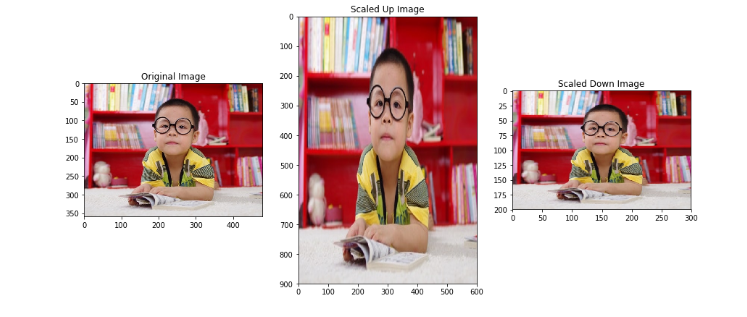
\includegraphics[width=500pt]{resizing1.png}
      \caption{Resizing an image using the first Method}
      \label{resizing1}
    \end{figure}

    \newpage

    \textbf{2) Specify a Scaling Factor:}\\
    This method is more useful when you want to resize the image but preserve the original aspect ration of the image. Here is the example code.

    \begin{center}
      \# Scaling Down the image 1.5 times by specifying both scaling factors\\
      scaleUpX = 1.5\\
      scaleUpY = 1.5\\

      \# Scaling Down the image 0.6 times specifying a single scale factor.\\
      scaleDown = 0.6\\

      scaledDown = cv2.resize(image, None, fx= scaleDown, fy= scaleDown, interpolation= cv2.INTER\_LINEAR)\\

      scaledUp = cv2.resize(image, None, fx= scaleUpX, fy= scaleUpY, interpolation= cv2.INTER\_LINEAR)\\
    \end{center}

    \begin{figure}[h]
      \centering
      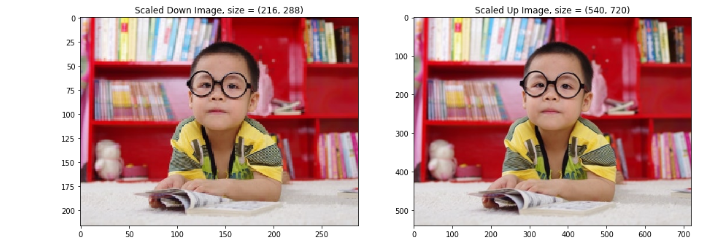
\includegraphics[width=250pt]{resizing2.png}
      \caption{Resizing an image using the second Method}
      \label{resizing2}
    \end{figure}

    As you can see the aspect ratio has not been disturbed as well as it is a lot easier to just do it this way. The only difference with doing it this way is that you have to do some quick math on what the change in aspect ratio should be.

    \subsubsection{Creating an Image Mask}
    Masking is a very important part of computer vision as it allows the program to ignore or highlight specific parts of the program based on certain conditions. \\
    I will now show how to create a mask based on pixel intensity or color.\\
    Lets say that we want to focus on creating a mask for the color red. Thinking about this logic is pretty simple and it just is that the red channel should have fairly high values (150+), and the other two channels should have low values (less than 100).\\
    The easiest way to do this is by using the OpenCV method called \textbf{inRnage}. This function takes an image and returns a binary image (black or white) based on the parameters that are passed into it.\\
    \textbf{Here is the syntax: }

    \begin{center}
      dst = cv2.inRange(src, lowerb, upperb[, dst])
    \end{center}

    \textbf{src: }the input array\\
    \indent\textbf{lowerb: }inclusive lower boundary array or a scalar\\
    \indent\textbf{upperb: }inclusive upper boundary array or a scalar\\
    \indent\textbf{dst: }output array of the same size as \textbf{src} and CV\_8U data type.

    \begin{center}
      mask2 = cv2.inRange(image, (0,0,150), (100,100,255))\\
      plt.figure(figsize=[15,15])\\
      plt.subplot(121);plt.imshow(image[...,::-1]);\\
      plt.title("Original Image")\\
      plt.subplot(122);plt.imshow(mask2);\\
      plt.title("Masked Image")\\
    \end{center}

    \begin{figure}[h]
      \centering
      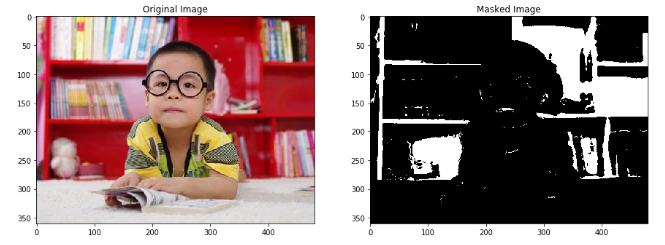
\includegraphics[width=200pt]{maskedimage.png}
      \caption{Masking the image based on red}
      \label{masking}
    \end{figure}


    \newpage

    \section{Matheatical Operations On Images}



\end{document}
